\section{Stratégie de développement}

\subsection{Paramètres d'étude}

Lors de la phase de développement, l'accent sera mis sur une production d'interface graphique simple, ergonomique et intuitive.
Le but est de fournir une application qui puisse être utilisée sans formation préalable, avec une installation la plus simple possible, sans sacrifier de fonctionnalité.

Afin de faciliter le développement de la plateforme de visualisation, cette dernière sera séparée en deux parties, comme les conventions de développement actuelles l'entendent. 
La partie dite \textbf{serveure} (backend) sera chargée des calcul et du rassemblement d'information. 
La partie dite \textbf{cliente} (frontend) sera, quant à elle, chargée de l'affichage des résultats.

Les utilisateurs verront uniquement la partie frontend, et selon les entrées spécifiés (les différents paramètres que les utilisateurs spécifieront), le frontend communiquera avec la partie backend pour que cette dernière effectue les calculs demandés, ou réunisse les informations nécessaires et les lui retourne.

\subsubsection{Ressources}

\textbf{Partie serveur} \\
Le langage envisagé pour la partie serveure est le Python.
Ce langage existe depuis 1991, et a été très largement adopté dans les communautés scientifiques.
Python bénéficie aujourd'hui d'un nombre impressionnant de librairies qui seront extrêmement pratiques pour la manipulation des données, les calculs ainsi que les rendus graphiques.
Pour créer le serveur qui permettra la connexion à une base de données ou les calculs divers, plusieurs choix sont possibles.
Django est un framework python largement utilisé dans tous les domaines.

En tant qu'alternative, la partie serveure pourrait aussi être développée en Ruby, un autre langage très utilisé pour les serveurs.
Le framework utilisé dans ce cas là serait Ruby on Rails.

\textbf{Partie cliente} \\
Pour la partie cliente, le développement se fera avec NextJS ainsi qu'avec NodeJS.
NextJS est un langage basé sur le TypeScript qui permet un grand contrôle sur la création d'interface et son comportement.
C'est un framework moderne, reconnu pour sa sécurité et largement adopté par des multinationales.
NodeJS est un framework JavaScript permettant de gérer des modules à ajouter à l'application (ici par exemple, les modules permettant la visualisation des graphiques, les modules de communications avec le backend, et d'autres).

\textbf{Base de données} \\
En termes de base de données pour le stockage des informations patients, il est judicieux d’opter pour une base de données locale (qui ne sera pas hébergée en ligne) écrite en SQLite.
Ce langage permet de créer des bases de données légère et rapides.
SQLite a été largement adopté pour tout type d’application nécessitant une base de données locale.

\subsubsection{Points bloquants}

\subsection{Protocoles établis}

\subsubsection{Prototype}
La plateforme de visualisation des signaux posturographique imaginée à été conçue 
pour être intuitive, simple d’utilisation ainsi que ergonomique facilitant au 
quotidien le diagnostic du médecin. Dès la page d’accueil, ce dernier peut accéder 
à l’ensemble de ses dossiers patients afin d’assurer un suivi personnalisé 
(Figure 6(a)). La plateforme permet également de visualiser les données 
enregistrées par la plateforme stabilométrique 
De plus, il est possible de visualiser les données 
(enregistrées par la plateforme stabilométrique) dans les domaines fréquentiels 
et temporels, tout en offrant la possibilité de sélectionner différents protocoles 
expérimentaux afin de comparer les résultats obtenus (Figure 6(b)). Le médecin a 
la possibilité d’ajuster différents paramètres, tels que la fréquence 
d’échantillonnage ou la durée d’observation des relevés de données.  Il dispose 
aussi d’un accès à des données synthétiques clés, comme la moyenne, la médiane ou 
l’écart-type, pour une analyse rapide (Figure 6(c)). Par ailleurs, la plateforme 
permet d’évaluer la stabilité du patient à travers divers examens cliniques, 
favorisant une corrélation entre les résultats cliniques et les données 
enregistrées. Enfin, chaque observation peut être exportée au format PDF à la fin 
de l’analyse, incluant les commentaires du médecin pour conserver une trace des 
conclusions tirées lors de l’étude.

\begin{figure}[H]
    \centering
    \begin{subfigure}[b]{0.45\textwidth}
      \hspace*{-2cm}
      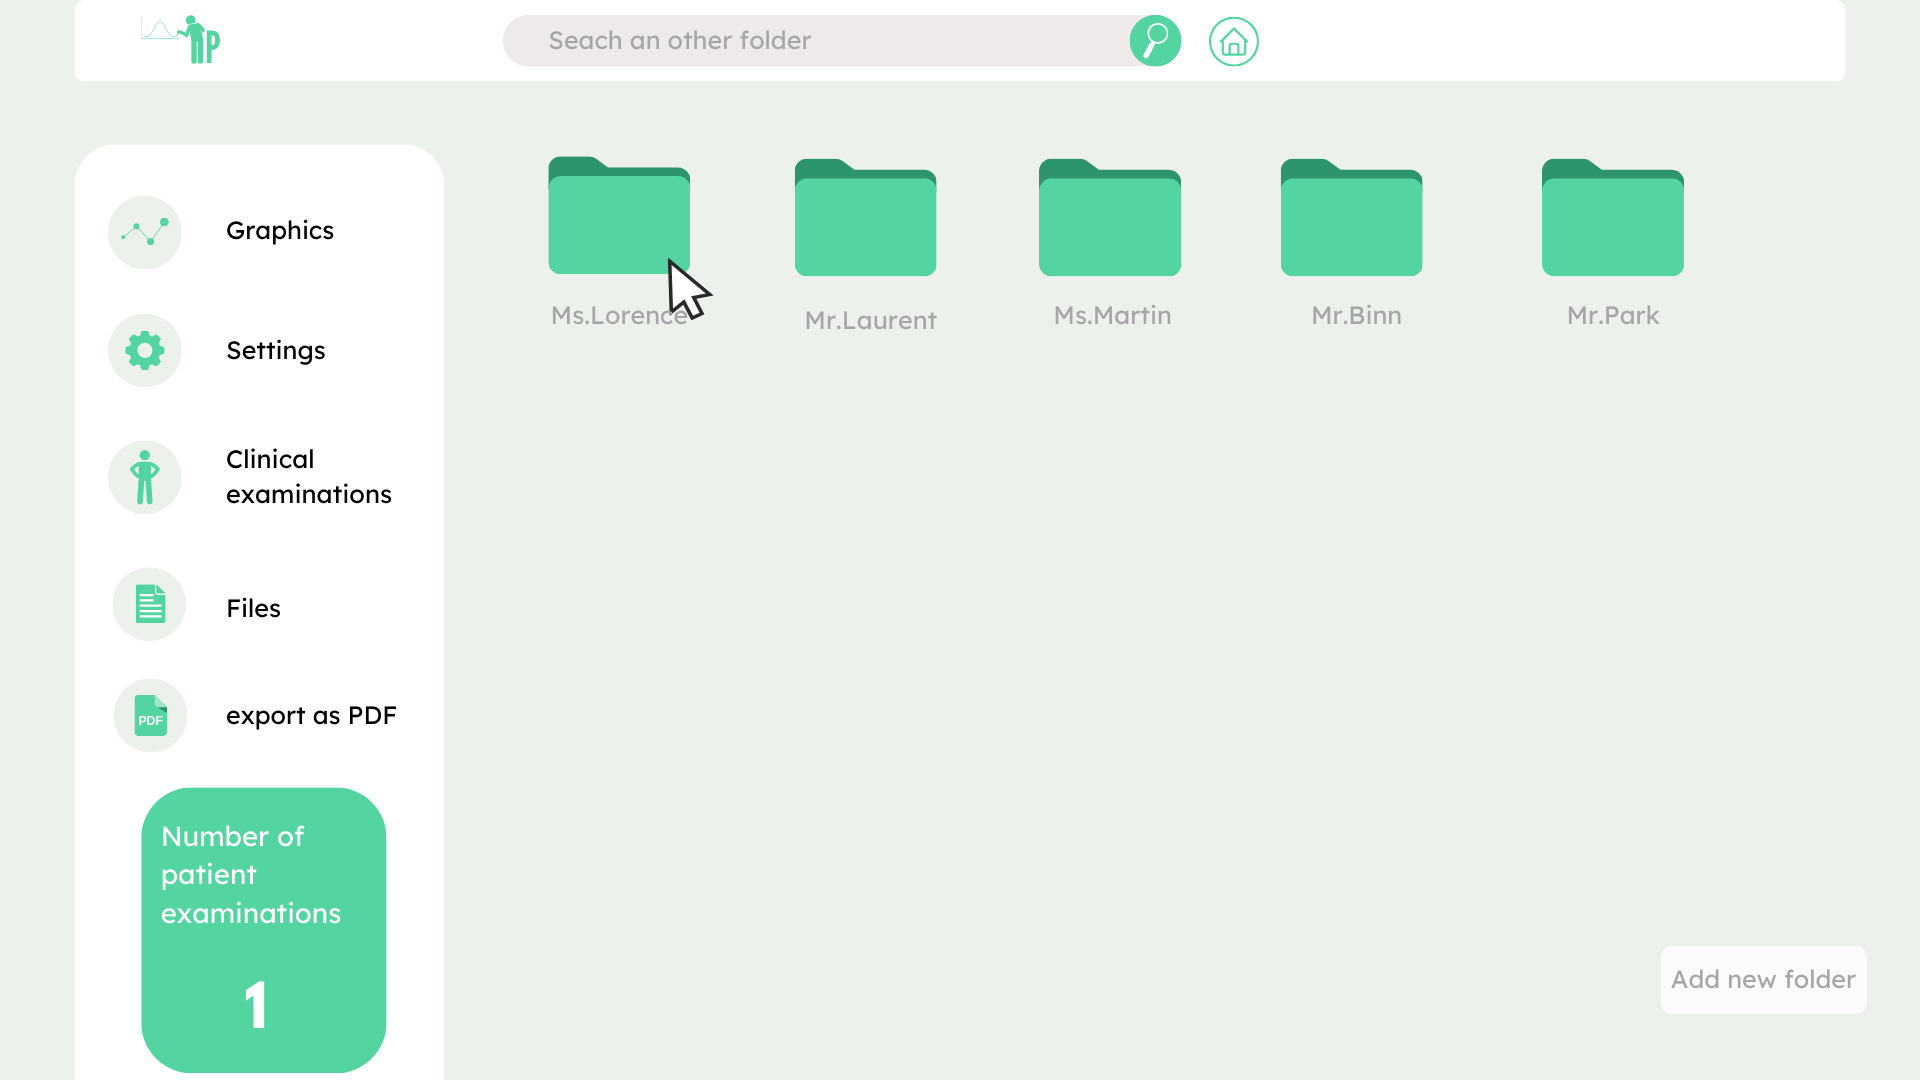
\includegraphics[height=5cm]{images/Prototype/Accueil de la plateforme de visualisation.png}
      \caption{Accueil de la plateforme de visualisation}\label{fig:Accueil de la plateforme de visualisation}
    \end{subfigure}
    \begin{subfigure}[b]{0.45\textwidth}
        \centering
      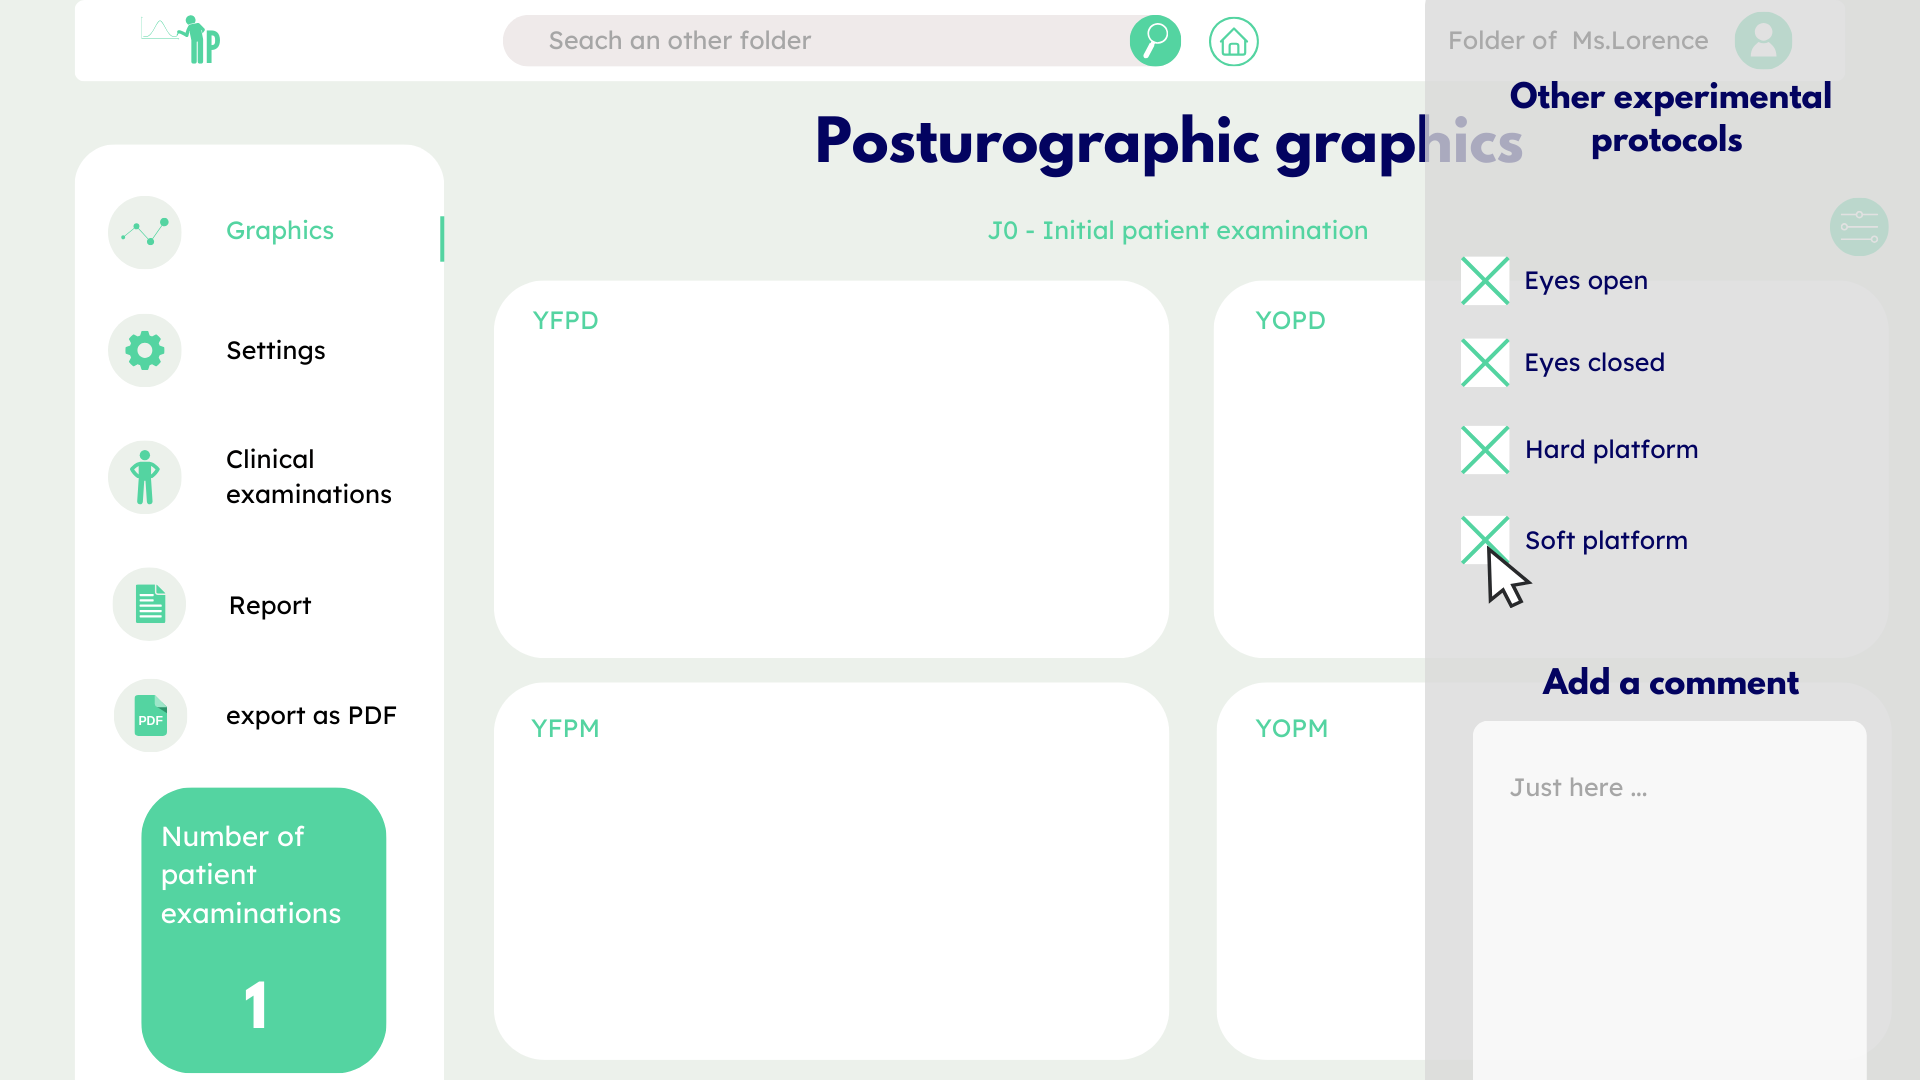
\includegraphics[height=5cm]{images/Prototype/Visualisation des données en fonction de différents protocoles expérimentaux.png}
      \caption{Visualisation des données en fonction de différents protocoles expérimentaux}\label{fig:Visualisation des données en fonction de différents protocoles expérimentaux}
    \end{subfigure}\\
    \begin{subfigure}[b]{0.45\textwidth}
      \centering
      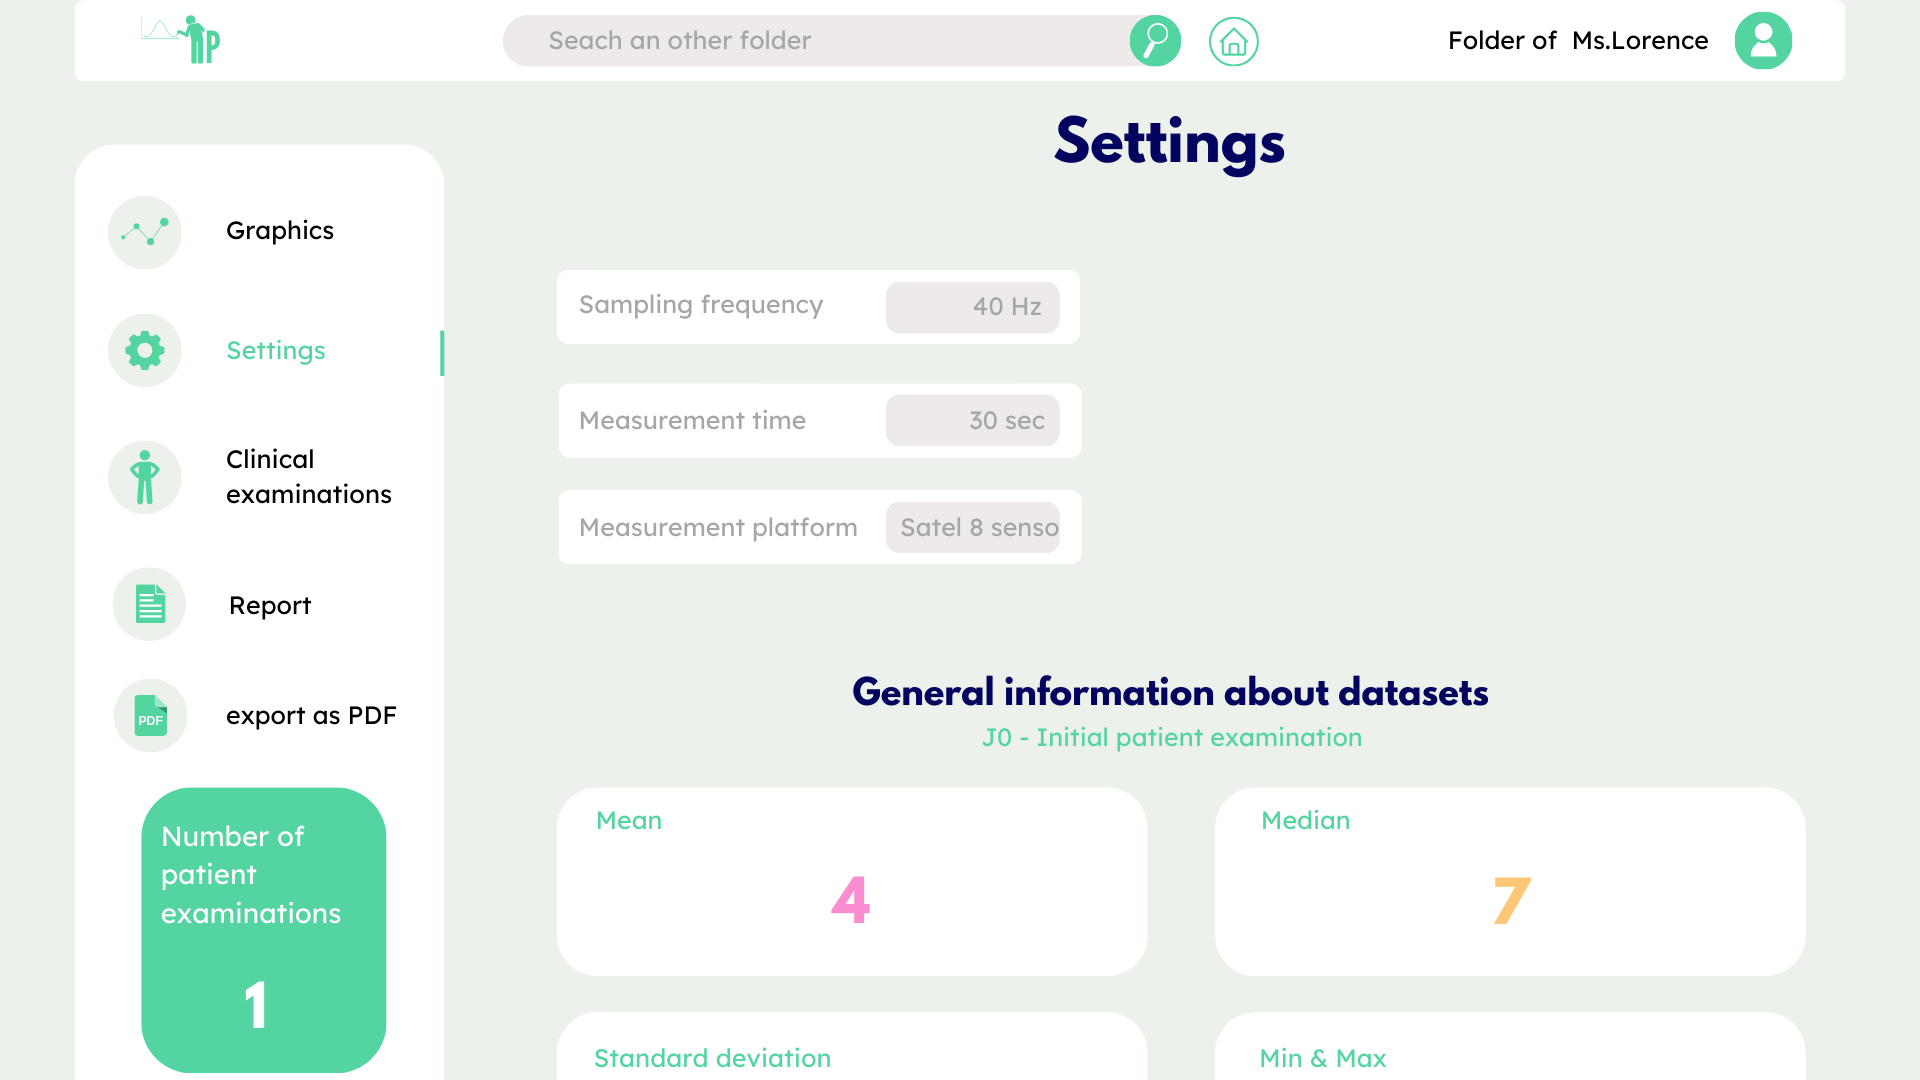
\includegraphics[height=5cm]{images/Prototype/visualiser des données clés du jeu de données étudié.png}
    \caption{visualiser des données clés du jeu de données étudié }\label{fig:visualiser des données clés du jeu de données étudié }
    \end{subfigure}
    \caption{Plateforme de posturographie imaginée}\label{fig:globalposturographie}
  \end{figure}